% -*-coding: utf-8 -*-
% Держать в начале каждого файла!

\documentclass[a4paper, 12pt]{extarticle}
\usepackage{metod}

\MTDSetPhysSection{Механика}
\MTDSetTitle{Измерение ускорения свободного падения с~помощью оборотного маятника}
\MTDDesignator{М--13}
\MTDSetGrade{10}

\MTDSetAuthors{И.~Н.~Грачева, В.~И.~Гребенкин, А.~Е.~Иванов, И.~А.~Коротова,
Е.~И.~Красавина, А.~В.~Кравцов, Н.~С.~Кулеба, Б.~В.~Падалкин,
Г.~Ю.~Шевцова, Т.~С.~Цвецинская}

\MTDSetEditorsGenCase{И.~Н.~Грачевой, А.~Е.~Иванова, А.~В.~Кравцова}

\newcommand{\eps}{\epsilon}
\newcommand{\isum}{\sum\limits_{i=1}^{n}}


\begin{document}

\MTDTitlePage
\MTDInfoPage

\setcounter{section}{13}

\subsection{Цель работы}
Целью работы является экспериментальное определение ускорения свободного падения.

\subsection{Основные теоретические сведения}
Физическим маятником называется твердое тело, имеющее возможность совершать колебания под действием силы тяжести вокруг неподвижной горизонтальной оси. Можно показать, что период малых свободных колебаний физического маятника определяется соотношением
\begin{equation}
\label{eq:m13-period}
T = 2 \pi \sqrt{\frac{I}{mgl}},
\end{equation}
где $g$ "--- ускорение свободного падения, $m$ "--- масса маятника, $I$ "--- момент инерции маятника относительно оси подвеса, $l$ "--- расстояние от оси подвеса до центра инерции маятника.

В частности, для математического маятника, масса которого сосредоточена в центре инерции, имеем $I_\text{м} = ml^2$. Тогда из равенства~\eqref{eq:m13-period} получаем
\begin{equation}
\label{eq:m13-math-pendulum-period}
T_\text{м} = 2 \pi \sqrt{\frac{l}{g}}.
\end{equation}

Соотношение~\eqref{eq:m13-period} удобно преобразовать, используя теорему
Штейнера
\begin{equation}
\label{eq:m13-steiner's-theorem}
I = I_0 + ml^2,
\end{equation}
где $I_0$ "--- момент инерции маятника относительно оси, проходящей через его центр инерции параллельно оси подвеса. Подставив равенство~\eqref{eq:m13-steiner's-theorem} в~\eqref{eq:m13-period}, находим
\begin{equation}
\label{eq:m13-period-2}
T = 2 \pi \sqrt{\frac{I_0 + ml^2}{mgl}}.
\end{equation}

Представляет интерес анализ зависимости периода~$T$ колебаний физического маятника от величины~$l$. В предельном случае больших значений $l$ соотношение~\eqref{eq:m13-period-2} переходит в~\eqref{eq:m13-math-pendulum-period}, т.~е. получаем математический маятник
\begin{equation}
\label{eq:m13-period-l-to-inf}
\left. T(l) \right|_{l \to \infty} = 2 \pi \sqrt{\frac{l}{g}}. %на самом деле ставить здесь прямую черту и стремление некорректно, так как потом l остается. правильно говорить, что при l много больше I_0... возможно, исходная косая черта это и значила, я не знаю. | Написать: "Когда $l >> I_0, соотношение~\eqref{eq:m13-period-2} переходит в~\eqref{eq:m13-math-pendulum-period}, т.~е. получаем математический маятник:", убрав "стремление" из формулы, аналогичено и для второго. Как тебе такое?
\end{equation}

При малых $l$ маятник близок к положению безразличного равновесия. В этом случае из соотношения~\eqref{eq:m13-period-2} получаем
\begin{equation}
\label{eq:m13-period-l-to-0}
\left. T(l) \right|_{l \to 0} = 2 \pi \sqrt{\frac{I_0}{mgl}}.
\end{equation}

Примерный вид графика зависимости $T(l)$ представлен на рис.~\ref{fig:m13-plot}. Асимптотическое поведение функции при $l \to \infty$ и $l \to 0$ описывается выражениями~\eqref{eq:m13-period-l-to-inf} и~\eqref{eq:m13-period-l-to-0}.  % И вот тут заменить на при $l >> I_0$ и $l << I_0$
Можно показать, что при $l_{\min} = \sqrt{I_0 / m}$ функция $T(l)$ имеет минимум. %степень 1/2 заменила на корень

\begin{figure}[h]
\begin{center}
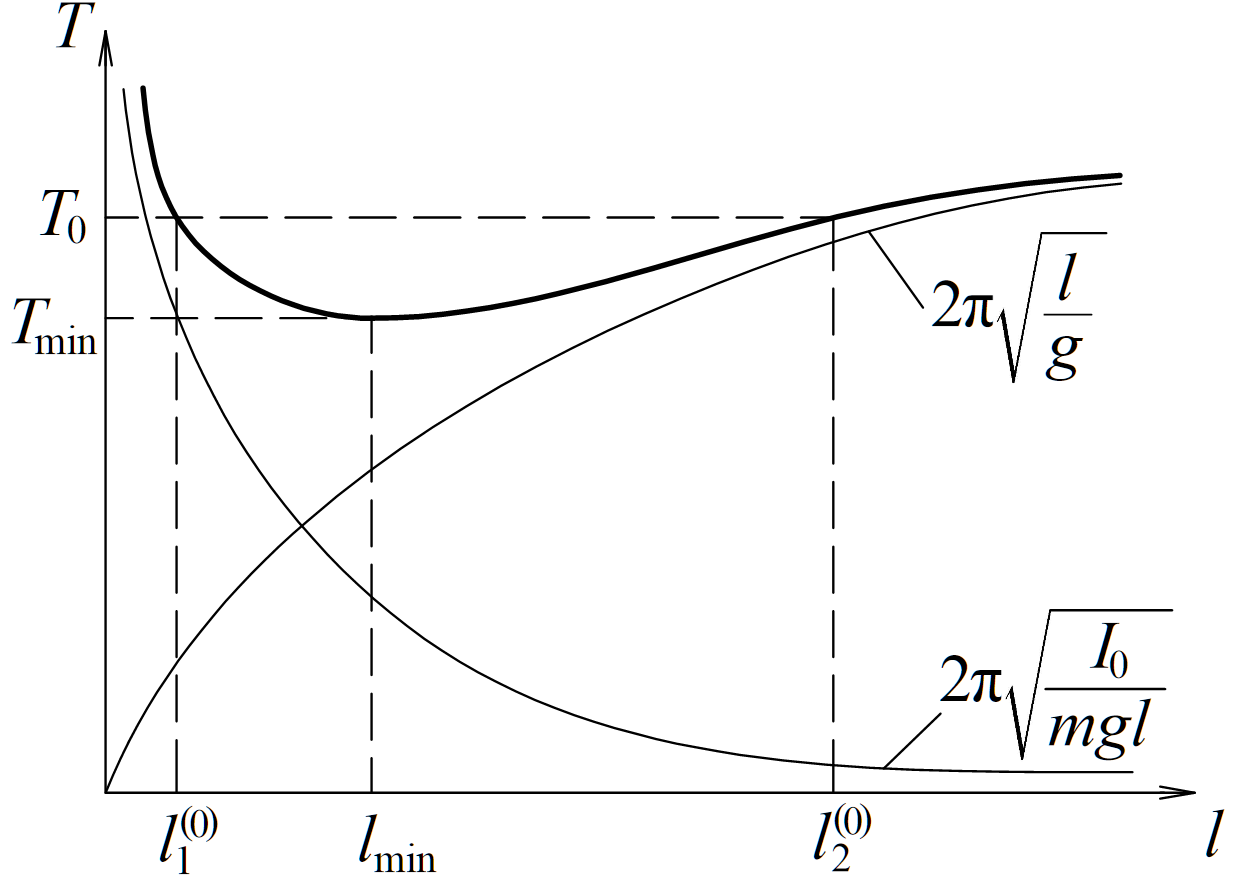
\includegraphics[width=0.5\linewidth, keepaspectratio=true]{M13-RotationalPendledumPeriods}
\end{center}
\caption{\label{fig:m13-plot}}
\end{figure}

Рассмотрим возможность определения с помощью физического маятника ускорения свободного падения $g$. Входящую в формулу~\eqref{eq:m13-period-2} величину $I_0$, которую трудно найти из опыта, можно исключить, измеряя период колебаний при двух разных значениях $l$. Записав равенство~\eqref{eq:m13-period-2} для $l_1$ и $l_2$, получим систему уравнений %ИЗМ: запятая после l_2
\begin{equation}
\label{eq:m13-system}
\left\{ \aligned
m g l_1 T_1^2 = 4 \pi^2 (I_0 + m l_1^2) \\
m g l_2 T_2^2 = 4 \pi^2 (I_0 + m l_2^2)
\endaligned \right.
\end{equation}
Отсюда находим
\begin{equation}
\label{eq:m13-g-1}
g = 4 \pi^2 \frac{l_1^2 - l_2^2}{T_1^2 l_1 - T_2^2 l_2}.
\end{equation}

На практике трудно точно определить положение центра инерции маятника, т.~е. измерить $l_1$ и $l_2$. Эту трудность можно обойти, если взять такие расстояния $l_1^{(0)}$ и $l_2^{(0)}$, чтобы соответствующие периоды были равны (см.~рис.~\ref{fig:m13-plot}), т.~е. выполнялось условие $T_1^{(0)} = T_2^{(0)} = T_0$. Тогда, полагая $l_1^{(0)} \ne l_2^{(0)}$, из равенства~\eqref{eq:m13-g-1} получаем %ИЗМ:запятая перед "чтобы''; запятая перез "из равенства"
\begin{equation}
\label{eq:m13-g-2}
g = \frac{4 \pi^2}{T_0^2} \left[ l_1^{(0)} + l_2^{(0)} \right] .
\end{equation}

При этом если оси расположены по разные стороны центра инерции, то сумма $l_1^{(0)} +l_2^{(0)}$ есть просто расстояние $l_0$ между осями, которое легко измерить с высокой точностью.

Итак, если наблюдается равенство периодов колебаний физического маятника относительно двух осей, находящихся по обе стороны центра инерции и на разном расстоянии от него, то величину $g$ можно найти из соотношения
\begin{equation}
\label{eq:m13-g-3}
g = 4 \pi^2 \frac{l_0}{T_0^2},
\end{equation}
где $l_0$  "--- расстояние между осями, $T_0$ "--- общий период колебаний.

\subsection{Описание экспериментальной установки}

\begin{figure}[h]
\begin{center}
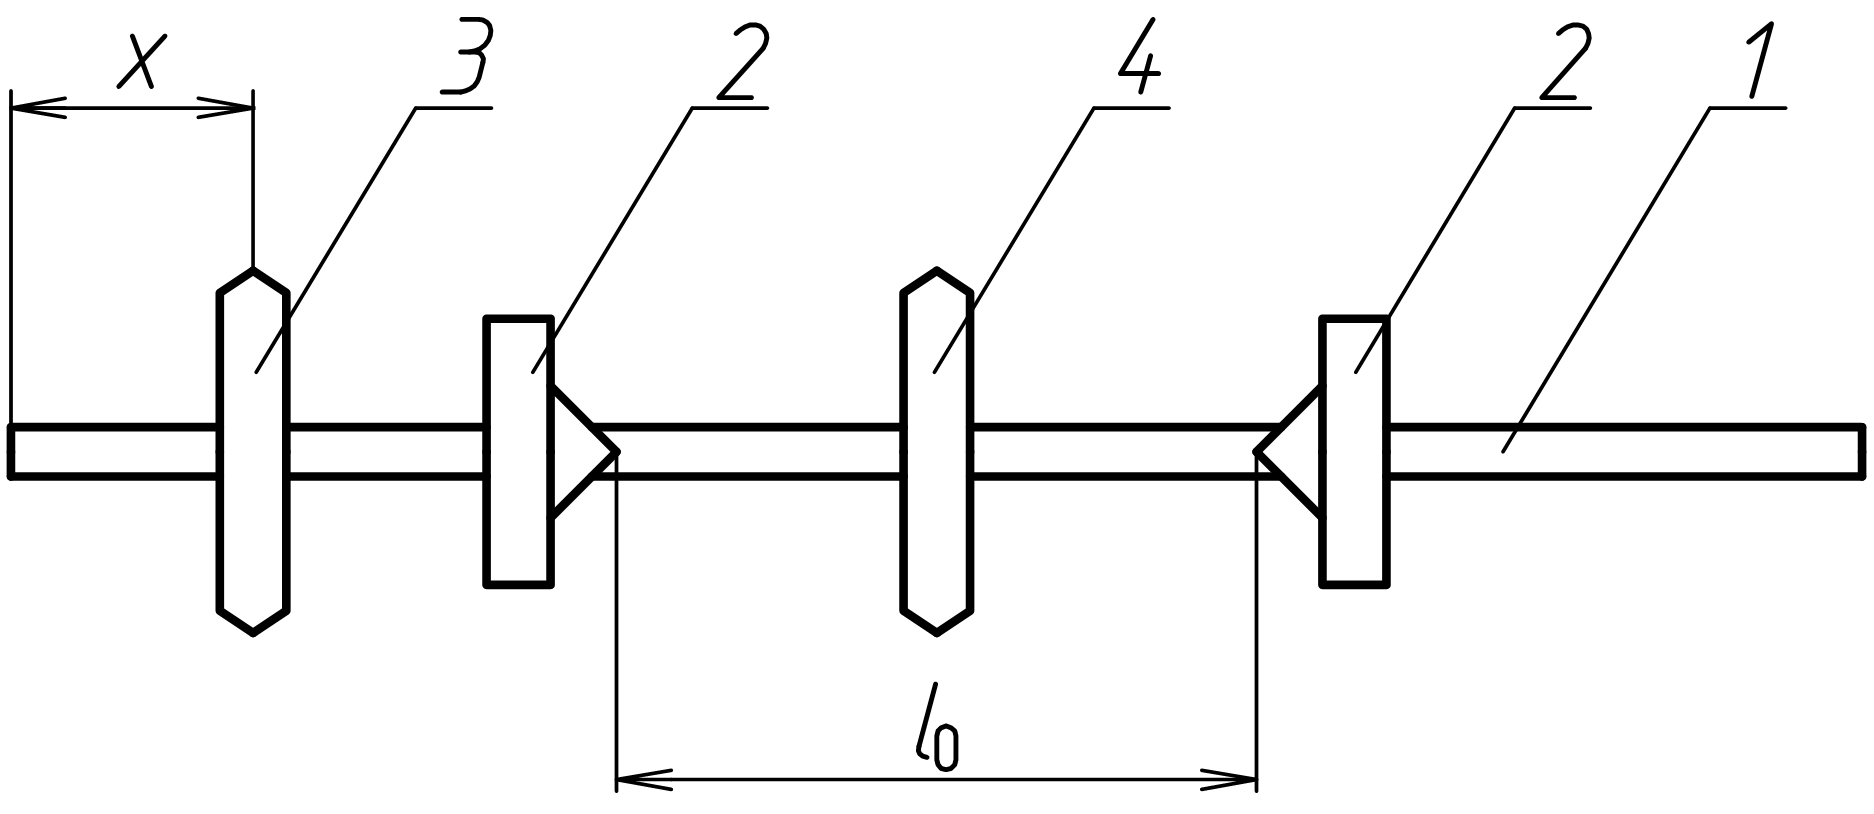
\includegraphics[width=0.5\linewidth, keepaspectratio=true]{M13-RotationalPendledum}
\end{center}
\caption{Схема оборотного маятника \label{fig:m13-pendulum}}
\end{figure}

В работе используется физический маятник, называемый оборотным. Схематически он изображен на рис.~\ref{fig:m13-pendulum}. Основной частью маятника является металлический стержень~\emph{1}. Осями подвеса служат ребра двух призм~\emph{2}, закрепленных вблизи концов стержня. В рабочем положении призмы устанавливаются в V-образные опоры штатива. %нужно ли вокруг V $? | Нет, это не формула.
Смещение центра инерции, необходимое для изменения расстояния $l_1$ и $l_2$,  обеспечивается перемещением массивного груза~\emph{3}, находящегося у конца стержня. Положение фиксированного груза~\emph{4} подобрано так, чтобы с помощью регулировочного груза можно было добиться равенства $T_1$ и $T_2$ в прямом и обратном положениях маятника.

Для более точного измерения величины $T_1^{(0)} = T_2^{(0)} = T_0$ в работе исследуется зависимость $T_1$ и $T_2$ от положения $x$ регулировочного груза, которое определяется по специальной шкале. Поскольку расстояние $l_0$ между осями фиксировано, то при смещении груза изменение $l_1$ и $l_2$ будет одинаково по величине, но противоположно по знаку. Как видно из рис.~\ref{fig:m13-plot}, это приведет к одинаковому по знаку изменению периодов $T_1$ и $T_2$. Однако при достаточной асимметрии в расположении центра инерции зависимость $T(x)$ в обратном положении маятника будет более крутой, чем в прямом. %видимо обратный и прямой надо местами поменять (судя по графику 1) | Пока не могу в это въехать, ещё потом подумаю

Таким образом, графики зависимостей $T_1(x)$ и $T_2(x)$ для прямого и обратного положений маятника будут иметь вид, изображенный на рис.~\ref{fig:m13-plot-2}. В результате значение $T_0$ можно найти как ординату точки пересечения соответствующих кривых. % не нужна ли запятая после "вид" и после "в результате"? | Первая нужна, причастный оборот, поставил, вторая не нужна, наречие, не требующее знаков препинания.

\begin{figure}[h]
\begin{center}
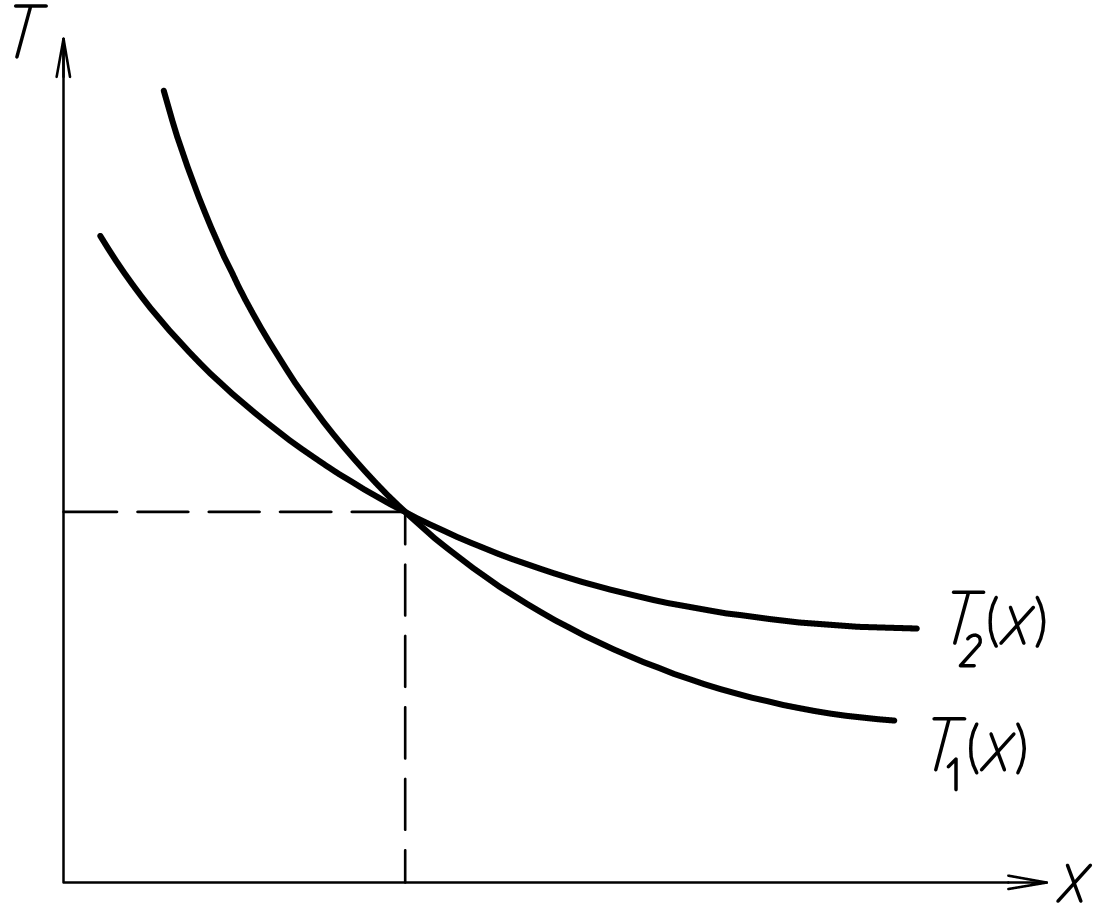
\includegraphics[width=0.4\linewidth, keepaspectratio=true]{M13-PeriodGraphIntersection}
\end{center}
\caption{Графики зависимостей $T_1(x)$ и $T_2(x)$ \label{fig:m13-plot-2}}
\end{figure}

Период колебаний маятника можно определить по формуле
\begin{equation}
\label{eq:m13-period-3}
T = \frac{t}{N},
\end{equation}
где $t$ "--- время, за которое совершается полное число $N$ колебаний.
При повторных измерениях удобно регистрировать время $t$ одного и того же числа колебаний $N$. Тогда нет необходимости сразу переходить к величине $T$.  Практически удобнее исследовать зависимости $t(x)$ для прямого и обратного положений маятника. Точка пересечения соответствующих графиков даст величину $ t_0 = t_1^{(0)} = t_2^{(0)}$. Тогда с учетом выражений~\eqref{eq:m13-g-3}, \eqref{eq:m13-period-3} получаем для расчета ускорения свободного падения соотношение %в последнем предложении где-то кажется нужны запятые или нет | Не нашёл, куда можно поставить. :)
\begin{equation}
\label{eq:m13-g-4}
g = 4 \pi^2 l_0 \left( \frac{N}{t_0}\right) ^2.
\end{equation}

Вследствие погрешностей измерений, экспериментальные точки на графике $t(x)$ могут не находиться на плавной кривой, предсказываемой теорией (см.~рис.~\ref{fig:m13-plot-2}). Поэтому при обработке результатов измерений кривые $t_1(x)$ и $t_2(x)$ следует провести приближенно, стремясь минимизировать их средние отклонения от полученных из опыта точек. % нужна ли запятая после "измерений" в 1-ом предложении? | Почитал грамоту.ру, скорее не нужно, чем нужно

\subsection{Порядок выполнения работы}

\begin{table}[h] %кажется, тут должна быть одна таблица на все, так как для каждого x измеряем t_1 и t_2. мне не хватает смелости это поменять | Я бы не менял... Вдруг им там советуют какие-то определённые значения брать, когда туда идут и обратно, и они разные, мы их расстроим...
\caption{\label{tab:m13-res-exp-1}}
\begin{center}
      \begin{tabular}{|>{\centering\arraybackslash} m{1.6cm}|>{\centering\arraybackslash} m{1.6cm}|>{\centering\arraybackslash} m{1.6cm}|>{\centering\arraybackslash} m{1.6cm}|>{\centering\arraybackslash} m{1.6cm}|>{\centering\arraybackslash} m{1.6cm}|}
      \hline
      \multirow{2}*{$x,~\Units{\text{см}}$} & \multirow{2}*{} & \multirow{2}*{} & \multirow{2}*{} &  \multirow{2}*{} &  \multirow{2}*{} \\ %сделала, что x в сантиметрах, мб лучше в метрах | Не, оставим сантиметры, "40" писать и говорить проще, чем "0,4"
      & & & & & \\ \hline
      \multirow{2}*{$t_1,~\Units{\text{с}}$} & \multirow{2}*{} & \multirow{2}*{} & \multirow{2}*{} &  \multirow{2}*{} & \multirow{2}*{} \\

	& & & & & \\ \hline
\end{tabular}
\end{center}
\end{table}

\begin{table}[h]
\caption{\label{tab:m13-res-exp-2}}
\begin{center}
      \begin{tabular}{|>{\centering\arraybackslash} m{1.6cm}|>{\centering\arraybackslash} m{1.6cm}|>{\centering\arraybackslash} m{1.6cm}|>{\centering\arraybackslash} m{1.6cm}|>{\centering\arraybackslash} m{1.6cm}|>{\centering\arraybackslash} m{1.6cm}|}
      \hline
      \multirow{2}*{$x,~\Units{\text{см}}$} & \multirow{2}*{} & \multirow{2}*{} & \multirow{2}*{} &  \multirow{2}*{} &  \multirow{2}*{} \\ %сделала, что x в сантиметрах, мб лучше в метрах
      & & & & & \\ \hline
      \multirow{2}*{$t_2,~\Units{\text{с}}$} & \multirow{2}*{} & \multirow{2}*{} & \multirow{2}*{} &  \multirow{2}*{} & \multirow{2}*{} \\
	& & & & & \\ \hline
\end{tabular}
\end{center}
\end{table}

\begin{enumerate}
\item При подготовке к выполнению работы следует установить стойку строго вертикально. Нижний конец стержня должен свободно проходить между окнами фотодатчика. Установить маятник так, чтобы регулировочный груз находился на расстоянии 2~\Units{см} от конца стержня.

\textbf{Внимание!} При работе с маятником следует соблюдать осторожность и убедиться, что ребро призмы, служащей осью подвеса, находится в углублении V-образной опоры. Амплитуда колебаний должна составлять около $10\,\Units{\degree}$. %я заменила "градусов" на обозначение | градусы страшно уехали

Измерить время $t_1$ для фиксированного $N$ от 10 до 15 полных колебаний маятника. Запуск и остановка секундомера осуществляется фотоэлектрическим датчиком. При нажатии на клавишу <<ПУСК>> начинается отсчет времени от момента прохождения маятником положения равновесия. При нажатии клавиши <<СТОП>> секундомер фиксирует длительность $t$ целого числа колебаний на момент ближайшего во времени прохождения маятником положения равновесия. Число колебаний фиксируется специальным индикатором. Записать значения $t$, $N$ и положение $x$ груза.
\item Перевернуть маятник и повторить задание п.~1. Определить время $t_2$.
\item Повторить опыт при четырех "--- пяти различных значениях $x$, перемещая груз из одного крайнего положения в другое. Для повышения точности, измерения при каждом $x$ повторить два "--- три раза. Результаты занесите в таблицы. %не знаю какой тут дефис | Я прочёл Лебедева и он говорит, что надо em-dash с пробелами, я заменил
\item Измерить расстояние $l_0$ между ребрами призмы, служащими осями подвеса маятника, и оценить его погрешность $\Delta l_0$.
\item При оформлении отчета построить графики зависимостей $t_1(x)$ и $t_2(x)$ для прямого и обратного положений маятника. Найти величину $t_0$ как   ординату  точки   пересечения соответствующих кривых. По формуле~\eqref{eq:m13-g-4} рассчитать величину $g$.
\item Оценить ошибку определения $t_0$ и рассчитать погрешность нахождения $g$.
\end{enumerate}

\subsection{Расчет погрешности}
Используя правила вычисления погрешности косвенных измерений, из выражения~\eqref{eq:m13-g-4} получаем следующую формулу для относительной погрешности величины $g$:
\begin{equation}
\label{eq:m13-error}
\frac{\Delta g}{g} = \sqrt{\left(\frac{\Delta l_0}{l_0}\right)^2 + 2 \left(\frac{\Delta t_0}{t_0}\right)^2},
\end{equation}
где $\Delta l_0$ и $\Delta t_0$ "--- абсолютные погрешности величин $l_0$ и $t_0$.

Поскольку расстояние $l_0$ измеряется непосредственно, то его погрешность определяется как обычно по данным многократных измерений.

Величина $t_0$ определяется косвенным методом по графикам зависимостей $t_1(x)$ и $t_2(x)$.  При этом вследствие наличия погрешностей $\Delta t$ при измерении времени $t$, график $t(x)$ фактически должен изображаться не линией, а полосой шириной около $2 \Delta t$. % нужна ли запятая после "времени t"? вроде бы можно заменить на "из-за" | Считаю, что надо, чтобы было "Из-за погрешностей $\Delta t$ при измерении времени $t$ график $t(x)$..."

Погрешность $\Delta t$ следует найти по данным многократных измерений промежутков времени $t$ и нанести на график. Тогда в результате пересечения  кривых $t_1(x)$ и $t_2(x)$, проведенных с учетом погрешности, получим некоторую область. Величина $t_0$ находится как ордината ее центра. Оценку погрешности $\Delta t_0$ получаем, учитывая, что максимальный размер указанной области вдоль оси ординат составляет $2 \Delta t_0$. При оценке $\Delta t_0$ следует учитывать, что точность построений на графике не превосходит~0,5~\Units{мм}. % нужно ли выделять "в результате"? | Грамота.ру говорит, что "обычно" "в результате" не выделяют, убрал оттуда запятую.

\subsection{Контрольные вопросы}
\begin{enumerate}
\item Дайте определение физического маятника.
\item Сформулируйте теорему Штейнера.
\item Каким образом задается и определяется значение $T_0$?
\item Что такое мгновенная ось вращения и чем она замечательна?
\end{enumerate}

\end{document} 